\documentclass[serif, xcolor={dvipsnames}]{beamer} % serif, mathserif


\definecolor{dodgerblue}{rgb}{0.12, 0.56, 1.0}
\definecolor{mygreen}{cmyk}{0.82,0.11,1,0.25}
\definecolor{aliceblue}{rgb}{0.94, 0.97, 1.0}

\definecolor{codegreen}{rgb}{0,0.6,0}
\definecolor{codegray}{rgb}{0.5,0.5,0.5}
\definecolor{codepurple}{rgb}{0.58,0,0.82}
\definecolor{backcolour}{rgb}{0.95,0.95,0.92}

\definecolor{bittersweet}{rgb}{1.0, 0.44, 0.37}
\definecolor{Gray}{gray}{0.85}
% \definecolor{LCyan}{rgb}{0.88,1,1}
\definecolor{mgreen}{rgb}{0.0,0.5,0.0}
%% \definecolor{mgreen}{rgb}{0.2, 0.8, 1}
\definecolor{brickred}{rgb}{0.8, 0.25, 0.33}
\definecolor{bleudefrance}{rgb}{0.19, 0.55, 0.91}
\definecolor{AB}{rgb}{0.94, 0.97, 1.0}
\definecolor{AB}{rgb}{0.9,.81,.68}
\definecolor{azureWeb}{rgb}{0.94, 1.0, 1.0}
\definecolor{beaublue}{rgb}{0.74, 0.83, 0.9}
\definecolor{linen}{rgb}{0.98, 0.94, 0.9}
\definecolor{magnolia}{rgb}{0.97, 0.96, 1.0}
\definecolor{moccasin}{rgb}{0.98, 0.92, 0.84}
\definecolor{navajowhite}{rgb}{1.0, 0.87, 0.68}
\definecolor{palecornflowerblue}{rgb}{0.67, 0.8, 0.94}


% \usepackage{fourier}
\usepackage{newunicodechar}
\newcommand\Warning{%
 \makebox[1.4em][c]{%
 \makebox[0pt][c]{\raisebox{.1em}{\small!}}%
 \makebox[0pt][c]{\color{red}\Large$\bigtriangleup$}}}%
\newunicodechar{⚠}{\Warning}

\usepackage{stackengine}
\usepackage{scalerel}
\newcommand\dangersign[1][2ex]{%
  \renewcommand\stacktype{L}%
  \scaleto{\stackon[1.3pt]{\color{red}$\triangle$}{\tiny !}}{#1}%
}



\usepackage{fontawesome} % lightbulb
% we can define where figures are located
\usepackage{enumerate}
\usepackage{etaremune} % reverse order for enumerate
\usepackage{hhline}
\usepackage{listings}
\newcommand{\idea}{{\faLightbulbO~}}
\newcommand{\Rq}{{\faSearch~}}

\newcommand{\xitem}{%
  \par\hangindent3em\hangafter0
  \noindent\llap{$\triangleright$\enspace}%
  \ignorespaces}
  
% \def\myitem{\hangindent=5em$\triangleright$}
\def\myitem{\hangindent=5em}


\usepackage[natbib=true,style=authoryear,backend=bibtex,useprefix=true,giveninits=true]{biblatex}
\addbibresource{./beamer_Refs.bib}
% \usepackage[backend=bibtex]{biblatex}
\DeclareNameAlias{author}{last-first}
% the following breaks long titles in References 
\DeclareFieldFormat[book,article]{title}{\textit{#1}}
\DeclareCiteCommand{\cite}
  {\color{cyan}\usebibmacro{prenote}}%
  {\usebibmacro{citeindex}%
   \usebibmacro{cite}}
  {\multicitedelim}
  {\usebibmacro{postnote}
  }


\usepackage[capitalise]{cleveref}

\def\code#1{{\scriptsize\texttt{#1}}}
% hypersetup only changes the year in citation.
\hypersetup{
    colorlinks=true,
    linkcolor=white, % color1 : will be black
    filecolor=red,
    urlcolor=ForestGreen,
    citecolor=cyan,
    bookmarksopen=false,
    pdftitle={Title},
    pdfauthor={Author},
}

\usepackage[scaled=.9]{helvet} % platino activation
\usepackage{tabularx,multirow}
\usepackage{colortbl}
\RequirePackage{booktabs}

\colorlet{shadecolor}{gray!40}

\usepackage{chngcntr}
\usepackage{tcolorbox}

\setbeamertemplate{footline}[text line]{}
\setbeamertemplate{navigation symbols}{}
\usepackage{subcaption}
\usepackage{amsmath}
\usepackage{amsthm}
\usepackage{amsfonts}
\usepackage{amssymb}
\usepackage{calrsfs}
\usepackage{multicol}
%\captionsetup{font={small,stretch=0.80}}
\DeclareCaptionLabelFormat{andtable}{#1~#2  \&  \tablename~\thetable}

\newtheorem{thm}{Theorem}[section] % "[section]" restarts the theorem counter at every new section.
\newtheorem{Coro}[thm]{Corollary}
\newtheorem{lem}[thm]{Lemma}
\newtheorem{rem}[thm]{Remark}
\newtheorem{exm}[thm]{Example}
\newtheorem{deff}{Definition}



\usepackage{textpos} % i donno what this does

% \usepackage{etoolbox}
% \usepackage{mathptmx}
\usepackage{graphicx}
% \usetheme{Berlin}


% \usetheme{Copenhagen}
% \usetheme{Ilmenau}
% \setbeamertemplate{blocks}[rounded][shadow=false]
% \addtobeamertemplate{block begin}{\pgfsetfillopacity{0.8}}{\pgfsetfillopacity{1}}

\usepackage{ulem}
\usepackage{cancel}
\usefonttheme{professionalfonts}
{\vspace*{.10mm}}
\usecolortheme{beaver}
\usetheme[height=10mm]{Boadilla} % adds date and page number
\usetheme[height=10mm]{Rochester}

\definecolor{beaver}{rgb}{0.6, 0.4, 0.2} % Define the beaver color in RGB
\setbeamercolor*{structure}{fg=mgreen}


\title{Making a Case}
\author{HN}
\institute[WSU]{Washington State University}
\date{\today}

\titlegraphic{
\includegraphics[width=.8cm]{cat1}}
%%%%%%%%%%%%%%%%
%%%%%%%%%%%%%%%% Fonts
\usepackage[osf, sc]{mathpazo}
% \renewcommand{\familydefault}{\sfdefault}
% \usepackage{lmodern}
% \usepackage{tgschola} % western type font
% \renewcommand{\familydefault}{\sfdefault} % nice
%\usepackage[sfdefault]{carlito}

%%%%%%%%%%%%%%%%%%%%%%%%%%%%%%%%%%%%%%%%%%%%%%%%%%%%%%%%%
\begin{document}
\maketitle

%\addtobeamertemplate{frametitle}{}{%}
%%%%%%%%%%%%%%%%%%%%
%%%%%%%%%%%%%%%%%%%%
%%%%%%%%%%%%%%%%%%%%

%%%%%%%%%%%%%%%%%%%%
%%%%%%%%%%%%%%%%%%%%
%%%%%%%%%%%%%%%%%%%%

\begin{frame}
\frametitle{General}

\begin{itemize}
\item Anything worth making needs patience and practice
\item If you want mastery, you need to immerse yourself in it till it becomes your second nature, just like walking

\vspace{.5in}
\item Top(?) two take aways from graduate school
\begin{enumerate}
\item Try not to have a bias/prejudice. be playful \Rq
\item When you are wrong, you are wrong \dangersign
\end{enumerate}
\end{itemize}
\end{frame}

%%%%%%%%%%%%%%%%%%%%%
%%%%%%%%%%%%%%%%%%%%%
%%%%%%%%%%%%%%%%%%%%%
\begin{frame}[t]
\frametitle{Source of This Notes}

\vspace{-.18in}
\begin{figure}[htbp]
    \centering
    \begin{minipage}{0.3\textwidth}
        \centering
        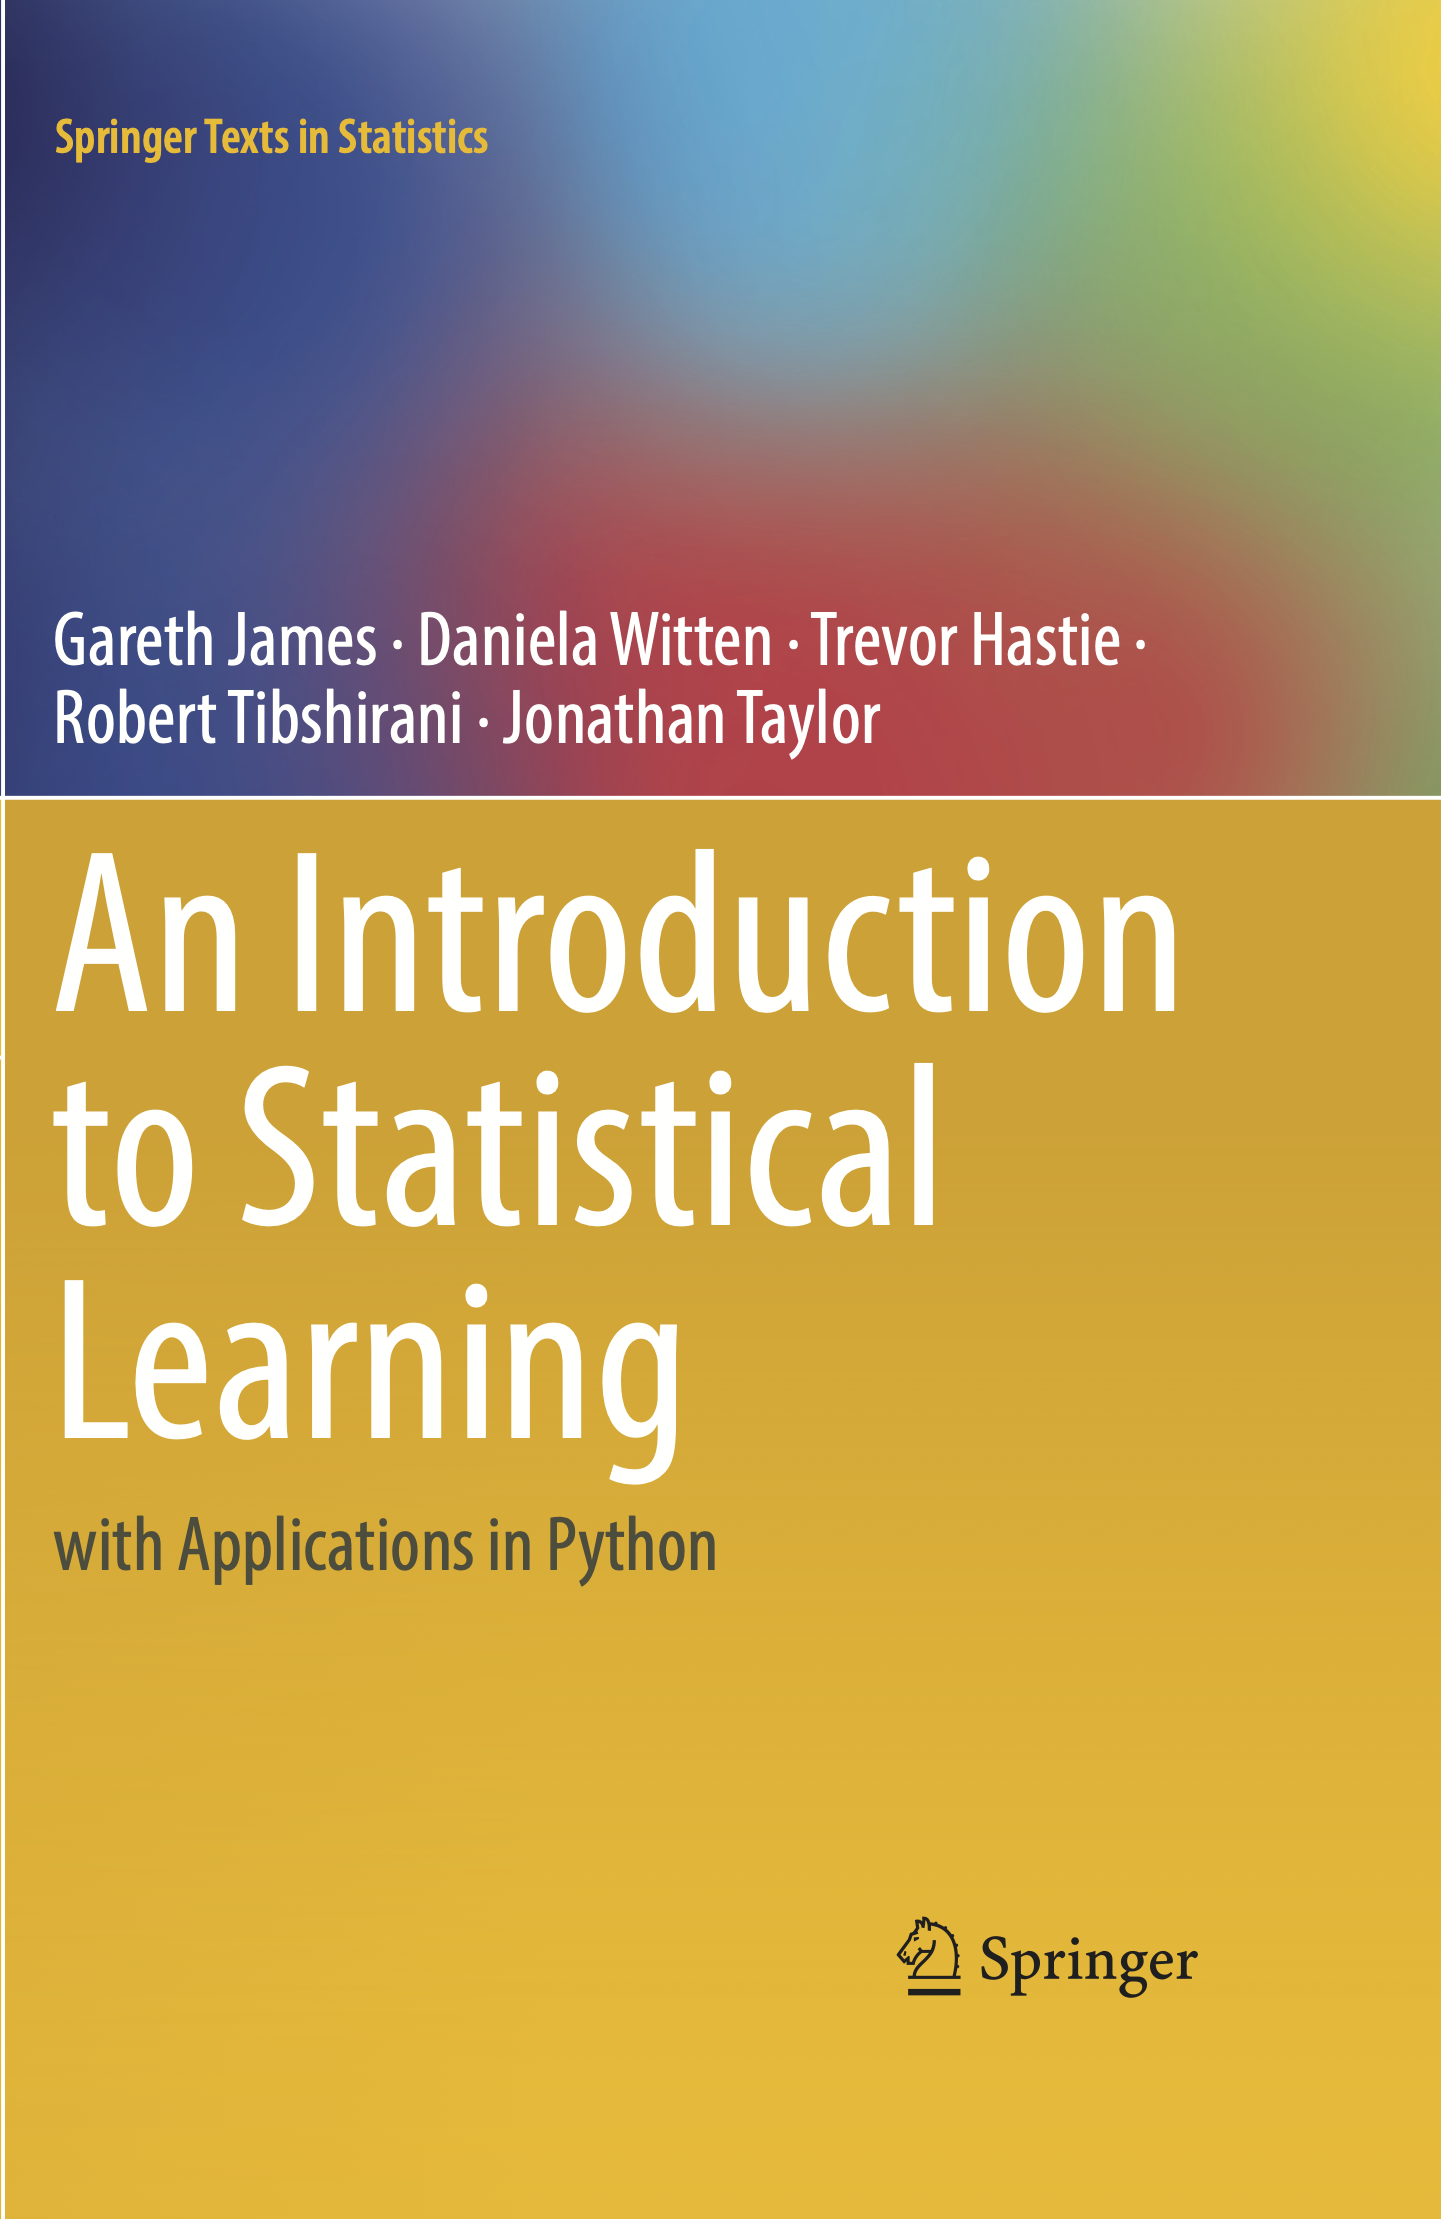
\includegraphics[width=\linewidth]{ISLP_cover}
    \end{minipage}%
    \hspace{.2in}
    \begin{minipage}{0.5\textwidth}
       Notes from\\ {\bf An Introduction to Statistical Learning} {\tiny with Applications in Python}
    \end{minipage}
\end{figure}

\begin{itemize}
\item It's an easy read and as the name suggests, it's just Introduction. Good for intuition building
\item Its PDF is available for free from the Authors' website.
\item Sign-up \& receive coupons (30\%-50\% off)
\end{itemize}

\end{frame}
%%%%%%%%%%%%%%%%%%%%%
%%%%%%%%%%%%%%%%%%%%%
%%%%%%%%%%%%%%%%%%%%%
\begin{frame}[t]
\frametitle{Last thing first (There is no magic wand)}

\begin{itemize}
\item There is no unique tool that outperforms other methods (there is no free lunch) 
\pause
\item There is no tool that is both accurate (in predicting) AND interpretable (unless we get lucky?!)
\end{itemize}
\pause

\begin{figure}[htbp]
\centering
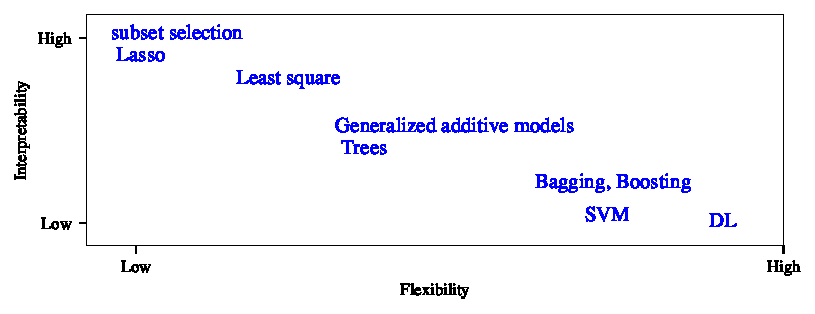
\includegraphics[width=\linewidth]{model_flex_inter}
\end{figure}
\end{frame}
%%%%%%%%%%%%%%%%%%%%%%%%%%%%%
%%%%%%%%%%%%%%%%%%%%%%%%%%%%%
%%%%%%%%%%%%%%%%%%%%%%%%%%%%%
\begin{frame}
\frametitle{Comparison of Model Performances}
\vspace{-.1in}
\begin{figure}[!ht] %htp
\captionsetup[subfigure]{labelformat=empty}
\centering
\hspace{-.12in}
\subfloat[]{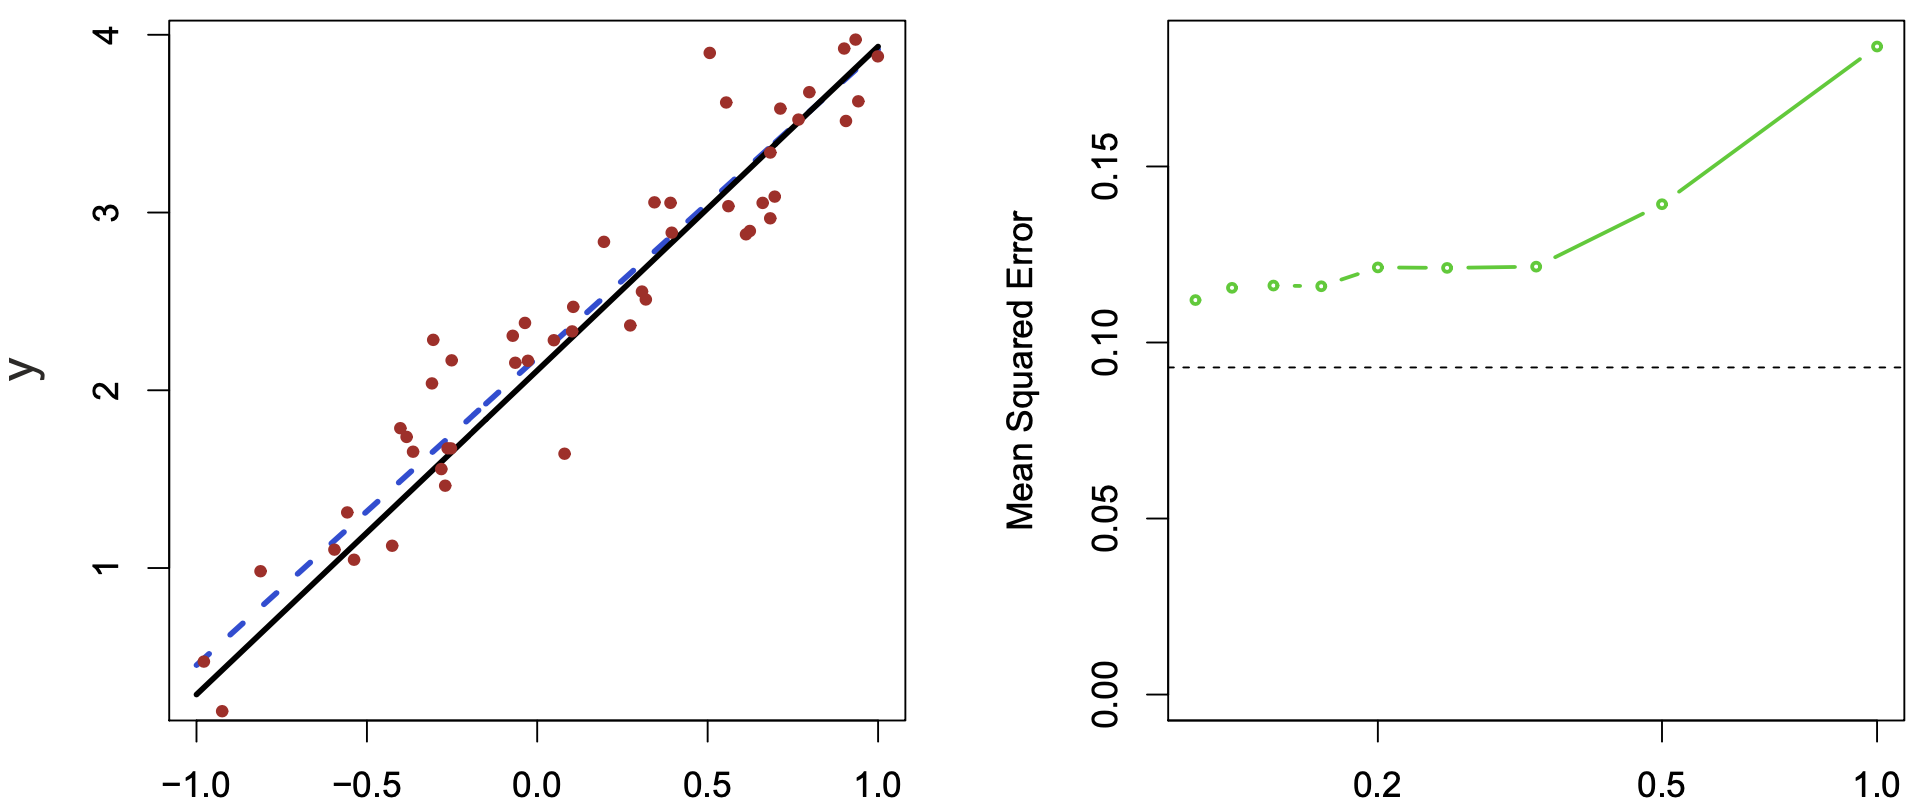
\includegraphics[width=.8\textwidth]{knnL}
}\\
\vspace{-.35in}
\subfloat[]{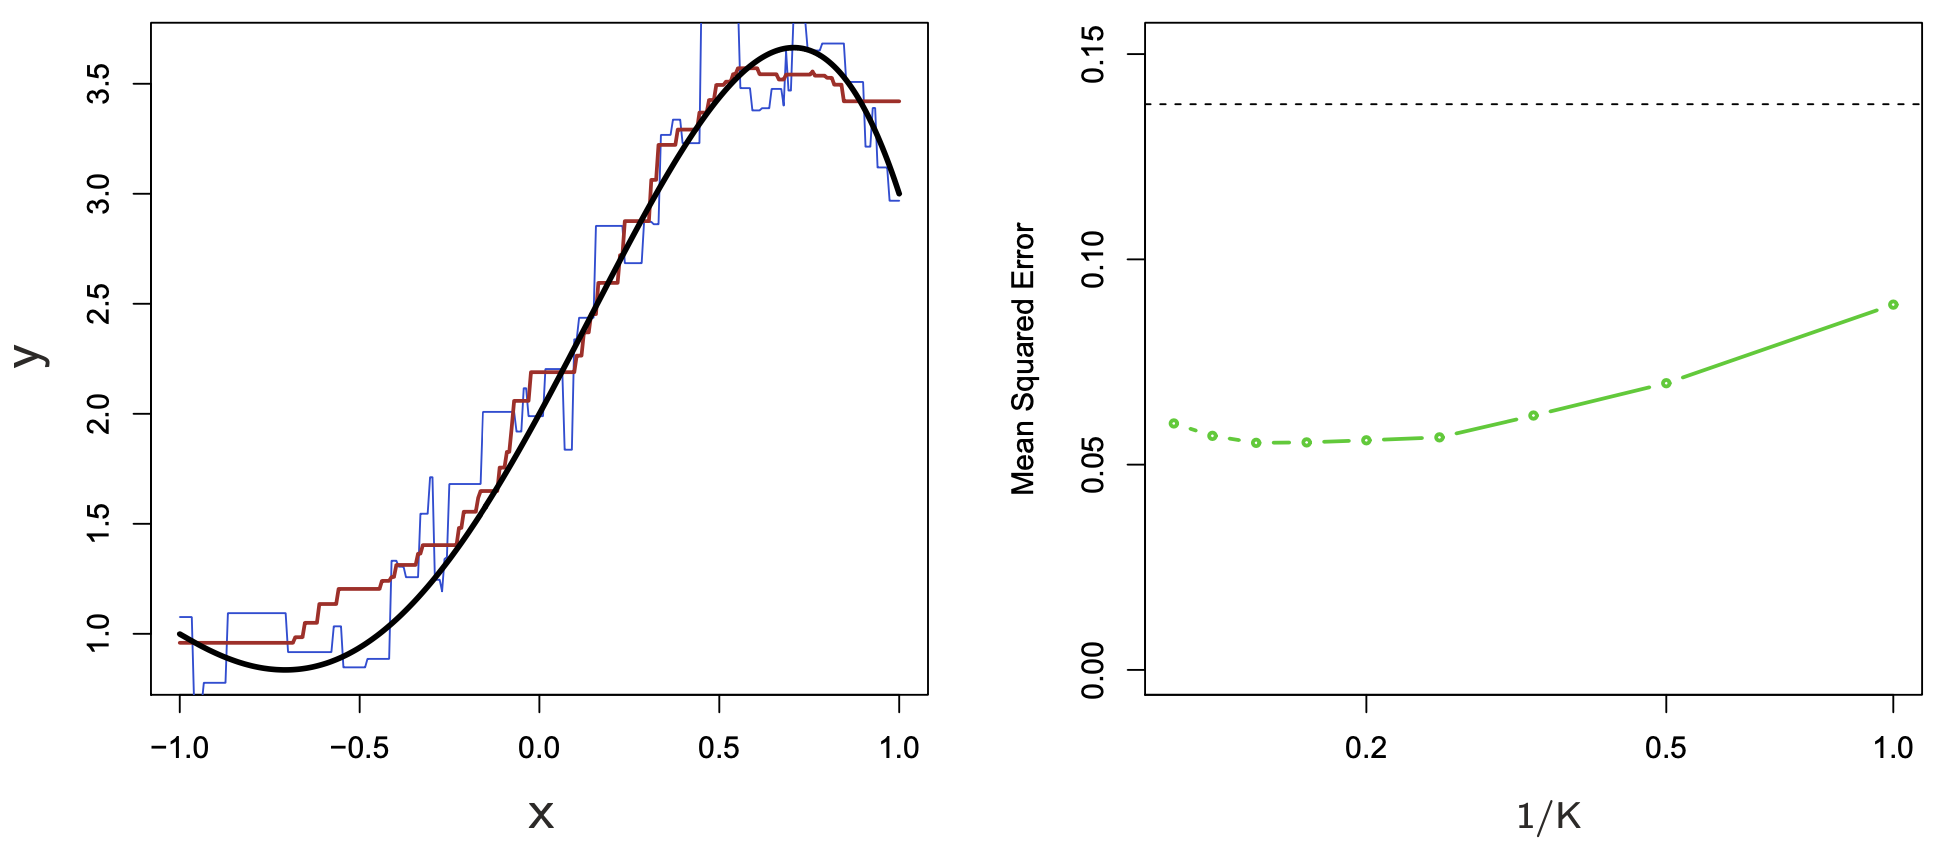
\includegraphics[width=.8\columnwidth]{knnNonL}
}
\end{figure}
\end{frame}

%%%%%%%%%%%%%%%%%%%%%%%%%%%%%
%%%%%%%%%%%%%%%%%%%%%%%%%%%%%
%%%%%%%%%%%%%%%%%%%%%%%%%%%%%
\begin{frame}
\frametitle{Some Model Assumptions}

\begin{itemize}
\item Logistic regression fits the data via likelihood maximization
\item Linear Discriminant Analysis (LDA): distribution of $X$ is normal in each class with identical covariance matrix.
\item Quadratic Discriminant Analysis (QDA): distribution of $X$ is normal in each class with class specific covariance matrix.
\end{itemize}
\end{frame}

%%%%%%%%%%%%%%%%%%%%%%%%%%%%%
%%%%%%%%%%%%%%%%%%%%%%%%%%%%%
%%%%%%%%%%%%%%%%%%%%%%%%%%%%%
\begin{frame}
\frametitle{Comparison of Model Performances}
\vspace{-.1in}
\begin{figure}[!ht] %htp
\captionsetup[subfigure]{labelformat=empty}
\centering
\subfloat[]{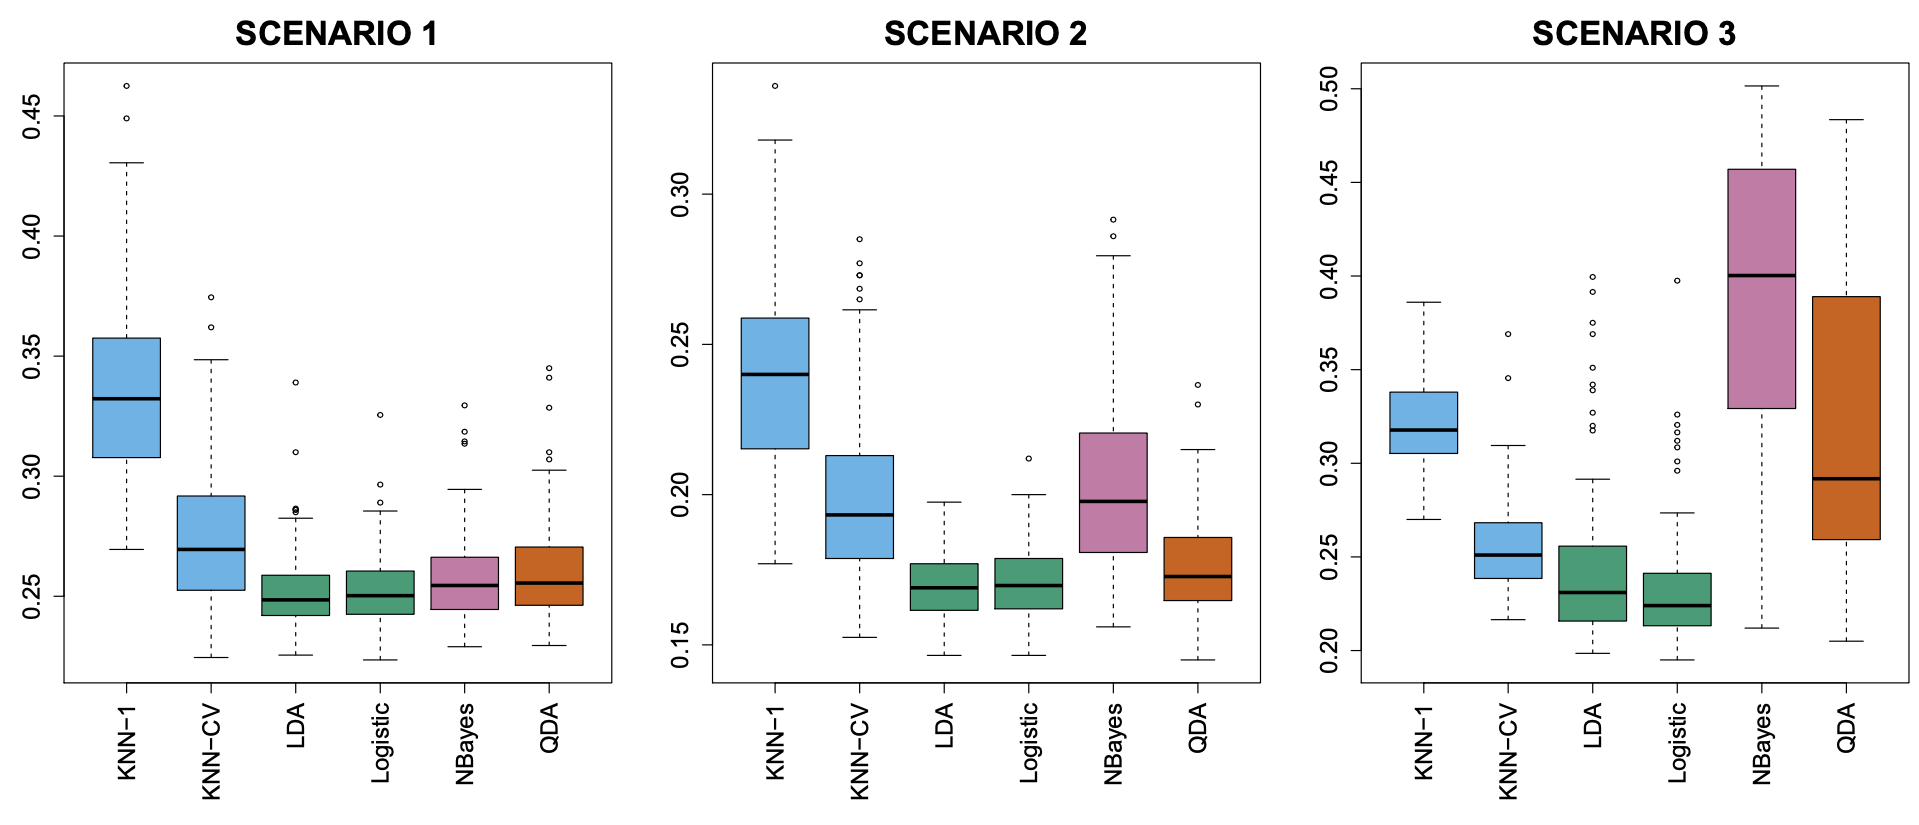
\includegraphics[width=.8\textwidth]{classification_compare}
}\\
\vspace{-.35in}
\subfloat[]{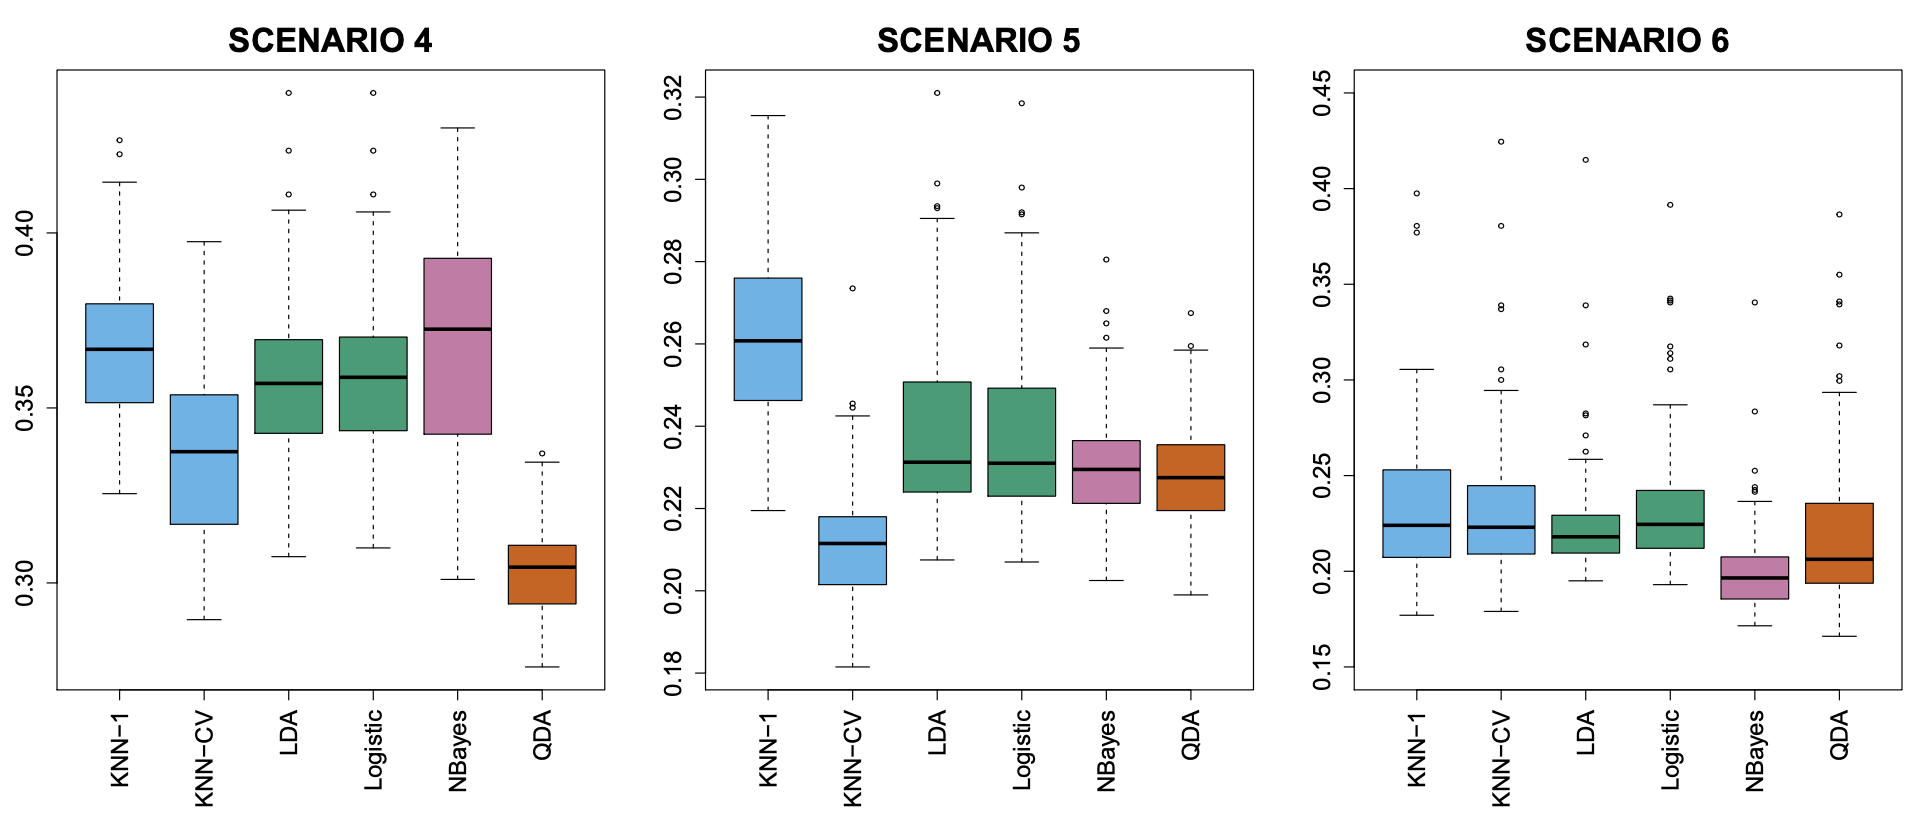
\includegraphics[width=.8\columnwidth]{classification_compare2}
}
\end{figure}
\end{frame}
%%%%%%%%%%%%%%%%%%%%%%%%%%%%%
%%%%%%%%%%%%%%%%%%%%%%%%%%%%%
%%%%%%%%%%%%%%%%%%%%%%%%%%%%%
\begin{frame}
\frametitle{PCR vs. PLS}
Two methods for reducing the dimensionality in regression

\begin{itemize}[<+->]
\item $y = {\color{dodgerblue}\mathbf{X}}\beta$
\item Principal Components Regression (PCR): regression using PCA
\item Partial Least Squares (PLS)
\item ``PLS is popular in the field of chemometrics \dots 
In practice it often performs no better
than ridge regression or PCR. While the supervised dimension reduction
of PLS can reduce bias, it also has the potential to increase variance, so
that the overall benefit of PLS relative to PCR is a wash.''
\end{itemize}
\vfill
\only<.(1)>{
{\bf Other uses of PCA}
\begin{enumerate}
\item Missing value imputation
\item Recommender systems
\item EDA
\end{enumerate}
}
%Ax = b \text{~~~~or~~~~} 
\end{frame}
%%%%%%%%%%%%%%%%%%%%%%%%%%%%%
%%%%%%%%%%%%%%%%%%%%%%%%%%%%%
%%%%%%%%%%%%%%%%%%%%%%%%%%%%%
\begin{frame}
\frametitle{a Note on p-value}
\begin{tcolorbox}
``\dots, p-values have recently been the topic of 
extensive commentary in the social science research community, to the extent
that some social science journals have gone so far as to ban the use of
p-values altogether! We will simply comment that when properly 
understood and applied, p-values provide a powerful tool for drawing inferential
conclusions from our data.''
\end{tcolorbox}

\begin{tcolorbox}
`` \dots By contrast, if we fail to reject $H_0$,
then our findings are more nebulous: we will not know whether we failed
to reject $H_0$ because our sample size was too small (in which case testing
$H_0$ again on a larger or higher-quality dataset might lead to rejection), or
whether we failed to reject $H_0$ because $H_0$ really holds.'' \\P. 559 (and read page 564).
\end{tcolorbox}
\end{frame}
%%%%%%%%%%%%%%%%%%%%%%%%%%%%%
%%%%%%%%%%%%%%%%%%%%%%%%%%%%%
%%%%%%%%%%%%%%%%%%%%%%%%%%%%%

%%%%%%%%%%%%%%%%%%%%%%%%%%%%%
%%%%%%%%%%%%%%%%%%%%%%%%%%%%%
%%%%%%%%%%%%%%%%%%%%%%%%%%%%%

%%%%%%%%%%%%%%%%%%%%%%%%%%%%%
%%%%%%%%%%%%%%%%%%%%%%%%%%%%%
%%%%%%%%%%%%%%%%%%%%%%%%%%%%%

%%%%%%%%%%%%%%%%%%%%%%%%%%%%%
%%%%%%%%%%%%%%%%%%%%%%%%%%%%%
%%%%%%%%%%%%%%%%%%%%%%%%%%%%%
\begin{frame}[t]
\frametitle{$R^2$}
\begin{itemize}[<+->]
\item True model $ y = f(x) + \varepsilon$\\
\item Our model $ y = \beta_0 + \beta_1x + \varepsilon$\\
\item The error term ($\sim N(0, \sigma^2)$) is a catch-all for what we miss with this
simple model: measurement errors, false modeling, omitted variables

\item RSS or $\text{RSE} = \sqrt{RSS/(n-2)}$ depend on Y-units. 

\item $R^2$ is unitless.

\item Small $R^2$ ``might occur because the linear model is wrong, or the error variance $\sigma^2$ is high, or both.''

\item ``\dots  and an $R^2$ value well below 0.1 might be more realistic!'' (page 79)
\end{itemize}
\end{frame}
%%%%%%%%%%%%%%%%%%%%%%%%%%%%%
%%%%%%%%%%%%%%%%%%%%%%%%%%%%%
%%%%%%%%%%%%%%%%%%%%%%%%%%%%%
\begin{frame}
\frametitle{General}

\begin{itemize}
\item Anything worth making needs patience and practice
\item If you want mastery, you need to immerse yourself in it till it becomes your second nature, just like walking

\vspace{.5in}
\item Top(?) two take aways from graduate school
\begin{enumerate}
\item Try not to have a bias/prejudice. be playful \Rq
\item When you are wrong, you are wrong \dangersign
\end{enumerate}
\end{itemize}
\end{frame}
%%%%%%%%%%%%%%%%%%%%%%%%%%%%%
%%%%%%%%%%%%%%%%%%%%%%%%%%%%%
%%%%%%%%%%%%%%%%%%%%%%%%%%%%%
\begin{frame}[t]
\frametitle{More Resources}

\begin{itemize}
\item {\scriptsize Guesstimation:~\citep{weinstein2008guesstimation}}
\item {\scriptsize First Course in Probability~\citep{ross1976first}}
\item {\scriptsize Introduction to Linear Regression Analysis~\citep{montgomery2021introduction}}
\end{itemize}
{\bf \scriptsize  Non-technical}
\begin{itemize}
\item {\scriptsize Excellent Sheep: The Miseducation of the American Elite and the Way to a Meaningful Life~\citep{sheep}}
\item {\scriptsize The Culture Code: The Secrets of Highly Successful Groups~\citep{CultureCode}}
\end{itemize}

{\bf \scriptsize  Tools}
\begin{itemize}
\item {\scriptsize Software Carpentry has lots of tutorials including \href{https://swcarpentry.github.io/git-novice/}{GitHub}!}
\end{itemize}
\end{frame}


%%%%%%%%%%%%%%%%%%%%%%%%%%%%%
%%%%%%%%%%%%%%%%%%%%%%%%%%%%%
%%%%%%%%%%%%%%%%%%%%%%%%%%%%%
\begin{frame}[allowframebreaks,t]{References} 
\frametitle{Some Definition}


\begin{deff}[Variance of a method] Variance refers to the amount by which
$\hat f$ would change if we estimated it using a different training data set.
\end{deff}
\pause
\begin{deff}[Bias of a method] Bias refers to the error that is introduced by approximating a real-life problem, which may be extremely complicated, by a much simpler model.
\end{deff}

\end{frame}

%%%%%%%%%%%%%%%%%%%%%%%%%%%%%
%%%%%%%%%%%%%%%%%%%%%%%%%%%%%
%%%%%%%%%%%%%%%%%%%%%%%%%%%%%

%%%%%%%%%%%%%%%%%%%%%%%%%%%%%
%%%%%%%%%%%%%%%%%%%%%%%%%%%%%
%%%%%%%%%%%%%%%%%%%%%%%%%%%%%
\begin{frame}[allowframebreaks, noframenumbering,t]
\frametitle{Bibliography}
\nocite{*}
\printbibliography

\end{frame}

\end{document}